\chapter{Variabili aleatorie}

\subsection{Introduzione}

Consideriamo uno spazio di probabilità $(\Omega, P)$. Spesso non siamo interessati a tutti i dettagli dell'esito dell'esperimento, ma solo a una \textit{quantità determinata dall'esito} dell'esperimento. Tale quantità è detta \textbf{variabile aleatoria}. \newline Una variabile aleatoria può essere descritta come una \textbf{funzione} $\Omega \xrightarrow{} \mathbb{R}$ \newline

\noindent \textbf{Osservazione}: Evento e variabile aleatoria sono diverse ma in relazione. Ogni variabile aleatoria mi permette di determinare più eventi. 
Sia X una variabile aleatoria e x un suo possibile valore: $\{X = x\}$ è un evento.\newline

\section{Variabili Aleatorie Discrete}

Una variabile aleatoria X si dice \textbf{discreta} se i valori che può assumere sono un insieme finito o un insieme infinito numerabile.  \newline Ad ogni variabile aleatoria discreta X possiamo associare un indice chiamato \textbf{Densità Discreta}: $$P_X(x_i) := P(X = x_i)$$

\subsubsection{Proprietà}
\begin{itemize}
    \item Se x non è un valore assunto da X, si pone $P_X(x) := 0$
    \item $P_X$ è una funzione da $\mathbb{R}$ a $[0,1]$
    \item $P_X(x_i) \geq 0$
    \item $\dsum_{i \geq 1} P_X(x_i) =1$
\end{itemize} 

\noindent \textbf{Osservazione}: La densità discreta ci risulta utile quando ci interessa sapere la densità di un sottoinsieme: $$P(X \in B) = \sum_{x_i \in B} P_X(x_i)$$ 

\begin{tcolorbox} 
    \textbf{Esempio}: Una pasticceria prepara 3 torte al giorno. Sappiamo che:
    \begin{itemize}
        \item il 20\% dei giorni nessun cliente ordina una torta
        \item il 30\% dei giorni un cliente ordina una torta
        \item il 35\% dei giorni due clienti ordinano una torta
        \item il restante dei giorni tre o più clienti ordinano una torta
    \end{itemize}
    Sia X il numero di torte invendute.
    \begin{enumerate}
        \item Qual è la densità discreta di X?        \item Qual è la probabilità q che il numero di torte invendute sia pari?
    \end{enumerate}
    Sappiamo che:
    \begin{itemize}
        \item $P_X(3) = P(X = 3) = 20\%$
        \item $P_X(2) = P(X = 2) = 30\%$
        \item $P_X(1) = P(X = 1) = 35\%$
    \end{itemize}
    Ricaviamo che $$P_X(0) = P(X = 0) = 1 - P(X = 3) - P(X = 2) - P(X = 1) = 15\%$$
    La probabilità che il numero di torte invendute sia pari è $$P_X(0) + P_X(2) = 45\%$$
\end{tcolorbox}

\newpage
\subsection{Valore Medio di Variabile Aleatoria Discreta}

Sia X una variabile aleatoria discreta. Si definisce \textbf{valore medio di X}: $$E[X] := \sum_{i=1}^N x_i \cdot p_X(x_i)$$

\subsubsection{Proprietà Valore Medio}

Per ogni variabile aleatoria X,Y e per ogni costante c $\in \mathbb{R}$ avremo:
\begin{itemize}
    \item \textit{Traslazione}: E[X + c] = E[X] 
    \item \textit{Moltiplicazione}: E[c $\cdot$ X] = c $\cdot$ E[X] 
    \item \textit{Somma}: E[X + Y] = E[X] + E[Y]
    \item \textit{Formula di trasferimento}: $E[f(x)] = \dsum_{i = 1}^N f(x_i) \cdot P_X(x_i)$
\end{itemize}

\noindent \textbf{Osservazioni}
\begin{itemize}
    \item Il valore medio è un operatore \textit{lineare}: $E[Z] = X + c$.
    \item \textit{Momento Secondo}: $E[X^2] = \dsum_{i=1}^N (x_i)^2 \cdot P_X(x_i)$
    \item Il valore medio E[X] non è necessariamente un valore $x_i$ assunto da X
    \item Il valore medio E[X] è quel valore tale per cui se ripetiamo un esperimento più volte, la media di tale esperimenti si avvicinerà a E[X]. Questo fenomeno è detto \textbf{Legge dei Grandi Numeri}: $$ \dfrac{\dsum_{i=1}x_i}{N} \simeq E[X]$$
\end{itemize}

\subsection{Varianza e Deviazione Standard}

Sia X una variabile aleatoria discreta e $\mu = E[X]$. Definiamo la \textbf{varianza} come: $$Var[X] := E[(X - \mu)^2]$$ A livello di calcolo, risulta più semplice utlizzare la formula: $$ Var[X] = E[X^2] - E[X]^2 $$

\noindent Definiano la \textit{deviazione standard} come: $$Sd[X] := \sqrt{Var[X]}$$

%\noindent La deviazione standard Sd[X] ha la stessa %unità di misura di X e fornisce una misura della %larghezza o dispersione dei valori $x_i$ ai assunti %da X rispetto al valore medio E[X]. \newline

%\noindent \textbf{Disuguaglianza di Chebyschev}: per %ogni t $>$ 0 avremo $$ P( |X - E[X] \geq t \cdot %Sd[X]) \leq \dfrac{1}{t^2}$$

\subsubsection{Propietà della Varianza}

Per ogni variabile aleatoria X  e per ogni costante c $\in \mathbb{R}$ avremo: 
\begin{itemize}
    \item Var[X + c] = Var[X]
    \item Var[c $\cdot$ X] = $c^2$ Var[X]
\end{itemize}

\begin{tcolorbox}
    \textbf{Esempio Completo}: Sia X il numero di figli maschi in una famiglia con due figli. Trovare: $P_X, E[X], Var[X], Sd[X]$ \newline
    \textit{Spazio Campionario} $$\Omega = \{MM, MF, FM, FF\}$$ 
    \textit{Densità Discreta} $$P_X(2) = {\dfrac{1}{4}}  \qquad P_X(1) = {\dfrac{1}{2}} \qquad P_X(0) = {\dfrac{1}{4}}$$
    \textit{Valore Medio} $$E[X] = 0 \cdot P(X = 0) + 1 \cdot P(X = 1) + 2 \cdot P(X = 2) = 1 \cdot \dfrac{1}{2} + 2 \cdot \dfrac{1}{4} = 1$$
    \textit{Momento Secondo} $$E[X^2] = 0^2 \cdot P(X = 0) + 1^2 \cdot P(X = 1) + 2^2 \cdot P(X = 2) = 1 \cdot \dfrac{1}{2} + 4 \cdot \dfrac{1}{4} = 1 \cdot \dfrac{3}{2} $$
    \textit{Varianza} $$ \text{Var[X]} = E[X^2] - E[X]^2= \dfrac{3}{2} - 1^2= \dfrac{1}{2}$$ 
    \textit{Deviazione Standard} $$ \sqrt{Var[X]} = \dfrac{1}{\sqrt{2}}$$
\end{tcolorbox}

\subsubsection{Variabili Indipendenti}

Siano X e Y due variabili aleatorie. Il valore della loro somma dipende da come sono "legate":
\begin{itemize}
    \item  Consideriamo Y = X. Allora Var[Y] = Var[X], quindi $$Var[X + Y]= Var[2X] = 4 \cdot Var[X]$$ 
    \item Consideriamo invece Y = -X. Allora $$Var[X + Y] = Var[X - X] = Var[0] = 0$$
\end{itemize}

\noindent Gli esempi precedenti sono casi estremi di dipendenza. Definiamo invece X e Y come variabili \textbf{indipendenti} se gli eventi \{X = x\} e \{Y = y\} sono indipendenti, ovvero $$P(X = x, Y = y) = P(X = x) \cdot P(Y = y)$$ 
\noindent \textbf{Definizione}: Se X e Y sono indipendenti allora $$ Var[X + Y] = Var[X] + Var[Y]$$

\section{Distribuzioni Notevoli Discrete}

Consideriamo una variabile aleatoria X in un certo esperimento aleatorio: $X : \Omega \xrightarrow{} \mathbb{R}$. Possiamo calcolare P($X \in A$) per ogni $A \subseteq \mathbb{R}$.
L'insieme di tali probabilità definisce la \textbf{Distribuzione della variabile aleatoria X}. \newline

\noindent \textbf{Osservazione}: Per variabili aleatorie discrete, la distribuzione di X è determinata dalla densità discreta e quindi, con abuso di notazione, si può dire che la distribuzione è la densità discreta.

\subsection{Bernoulli}

Variabile aleatoria X che può assumere soltanto i valori 0 e 1. Scriveremo \newline X $\sim$ Be(p). Sia p := (X = 1). Dato che $$\sum_{i=1}^{N} P_X(x_i) = P_X(0) + P_X(1) = 1$$ si ottiene:
\begin{equation}
  P(X = x) =
    \begin{cases}
      p & \text{se x = 1 }\\
      (1 - p) & \text{se x = 0 }\\
    \end{cases}       
\end{equation}


\noindent Allora, nel caso della variabile aleatoria di Bernoulli troviamo che:
\begin{itemize}
    \item Il \textbf{valore medio} E[X] = p.
    \item La \textbf{varianza} Var[X] = p(1 - p)
\end{itemize}

\subsection{Binomiale}

Consideriamo un esperimento aleatorio costituito da prove ripetute ed indipendenti dove abbiamo solo due esiti. Siano n il numero di prove e p la probabilità di successo di ciascuna e X il numero di successi. \newline La distribuzione di X è detta \textbf{binomiale} di parametri n e p indicata con \newline X $\sim$ Bin(n, p).  La densità discreta è data da: $$ P(X = k) = \binom{n}{k} \cdot p^k \cdot (1 -p)^{n - k} $$
dove:
\begin{itemize}
    \item P(X = k) è esattamente il numero k di successi in n prove
    \item $p^k$ è la probabilità di k successi fissati
    \item $(1 - p)^{n-k}$ è la probabilità di (n - k) insuccessi fissati
    \item $\binom{n}{k}$ scelte di quali prove hanno successo
\end{itemize}
\noindent Introduciamo le variabili:
\begin{equation}
  X_i =
    \begin{cases}
      1 & \text{se la i-esima prova ha successo}\\
      0 & \text{se la i-esima prova non ha successo}\\
    \end{cases}       
\end{equation}
Possiamo allora scrivere: $$ X = \sum_{i=1}^{N} X_i$$
Avremo che ogni $X_i \sim Be(p)$ e quindi sappiamo valore medio e varianza. Otteniamo allora:
\begin{itemize}
    \item \textbf{Valore medio} E[X] =$ n \cdot p$
    \item \textbf{Varianza} Var[X] = $n \cdot p \cdot (1 - p)$
\end{itemize}

\begin{tcolorbox}
    \textbf{Esempio}: Sia X numero di figli maschi in una famiglia con 2 figli.  
    Abbiamo $\Omega = \{MM, MF, FM, FF\}$ e avremo : $$P_X(0) = {\dfrac{1}{4}}  \qquad P_X(1) = {\dfrac{1}{2}} \qquad P_X(2) = {\dfrac{1}{4}}$$
    Allora X $\sim$ Bin(2; $\dfrac{1}{2})$: $$P_X(k)= \binom{2}{k} \cdot \dfrac{1}{2}^k \cdot \dfrac{1}{2}^{2 - k}= \dfrac{2}{k! \cdot (2 - k)!} \cdot \dfrac{1}{2^2} = \dfrac{1}{2} \cdot \dfrac{1}{k! \cdot (2-k)!} $$
    Infatti, se sostituiamo k=0, ritroveremo $P_X(0) = \dfrac{1}{4}$, se k=1 avremo $P_X(1) = \dfrac{1}{2}$ e con k=3 avremo $P_X(2) = \dfrac{1}{4}$
\end{tcolorbox}

\subsection{Poisson}

Una variabile aleatoria X si dice di Poisson di parametro $\lambda \in (0, \infty)$ ovvero X $\sim Pois(\lambda)$ se X($\Omega$) = $\mathbb{N}_0$ e $$P(X = k) = e^{- \lambda} \cdot \dfrac{\lambda^k}{k!}$$

\noindent \textbf{Approssimazione di Poisson}: Possiamo ottenere $X \sim Pois(\lambda)$ attraverso una variabile aleatoria binomiale $ Y \sim Bin(n,p)$ quando: $$ n \xrightarrow{} \infty \qquad p \xrightarrow{} 0 \qquad \text{allora } \quad n \cdot p = \lambda$$ 
Allora avremo che:
\begin{itemize}
    \item Il \textbf{Valore medio} E[X] = $\lambda$
    \item La \textbf{Varianza} Var[X] = $\lambda$
\end{itemize}

\noindent \textbf{Osservazione}: Le variabili aleatorie di Poisson sono approssimazioni per variabili aleatorie che contano il numero di successi quando si considera una grande quantità di prove la cui probabilità di successo è piccola. \newline

\begin{tcolorbox}
    \textbf{Esempio}: In un ospedale nascono mediamente 2,2 bambini ogni giorno. Qual è la probablità che nessun bambino nasca in ogni giorno. E qual è la probabilità che ne nascono più di 3? \newline
    Sia X il numero di nascite in un giorno. Supponiamo $ X \sim Pois(\lambda)$. Sappiamo che E[X] = $\lambda$ e per ipotesi E[X] = 2,2. calcoliamo:
    \begin{itemize}
        \item P(X = 0) = $e^{- \lambda} \cdot \dfrac{e^0}{0!} = e^{-2,2} \simeq 11\%$
        \item P(X $>$ 3) = 1 - P(X = 0) - P(X = 1) - P(X = 2) - P(X = 3) = $1 - e^{- \lambda} (1 + \lambda + \dfrac{\lambda^2}{2} + \dfrac{\lambda^3}{6}) = 18\% $
    \end{itemize}
\end{tcolorbox}

\subsection{Geometrica}

Una variabile aleatoria X si dice \textbf{Geometrica} di parametro p $\in$ (0, 1] e si scrive X $\sim$ Geo(p) se $$ P(X = k) = p \cdot (1- p)^{k-1} $$

\noindent \textbf{Osservazione}: Se p è 1, allora possiamo dire che, per quanto piccola sia la probabilità, l'evento prima o poi accadrà. \newline

\noindent Possiamo ottenere una variabile aleatoria geometrica partendo da una successione di prove ripetute dove consideriamo T l'istante del primo successo. Avremo che $$ P(T = k) = P(X_1 = 0, ..., X_{K - 1} = 0, X_K = 1) = (1 - p)^{k - 1} \cdot p$$ 

Allora troviamo:
\begin{itemize}
    \item il \textbf{Valore medio} E[X]= $\dfrac{1}{p}$
    \item la \textbf{Varianza} Var[X] = $\dfrac{1 - p}{p^2}$
\end{itemize}

\noindent \textbf{Osservazione}: Possiamo calcolare la probabilità di coda: $$P(T > n) = (1 - p)^n \qquad P(T \leq n) = \sum_{k=1}^N P_T(k) = (1 - p)^n$$

\newpage
\section{Var. Aleatorie Assolutamente Continue}

Consideriamo una classe complementare di variabili aleatorie, dette \textbf{assolutamente continue}, che assumono un insieme \textit{infinito più che numerabile di valori}, come ad esempio un intervallo in $\mathbb{R}$. \newline Una variabile X è assolutamente continua se la sua distribuzione è determinata da una funzione $f_X(x)$ a valori positivi detta \textbf{densità della variabile aleatoria X} nel modo seguente: $$P(X \in [s, t]) = \int_s^t f_X(x) dx $$

\begin{figure}[h!]
    \centering
    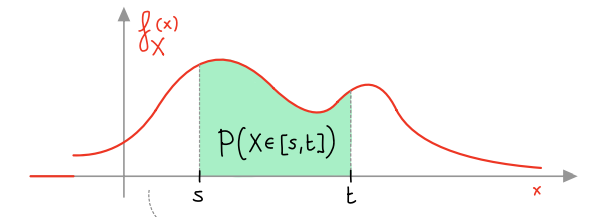
\includegraphics[scale=.7]{Foto/integrale.png} 
\end{figure}

\noindent \textbf{Osservazione}: Troviamo una analogia tra una variabile aleatoria discreta ed una assolutamente continua: $$ \text{V.A. discreta:} \sum_{x \in [s,t]} P_X(x_i) \qquad \text{V.A. assolutamente continua:} \int_s^t f_X(x) $$ 
 
\noindent Notiamo anche delle differenze importanti: se X è assolutamente continua $\forall x \in \mathbb{R}: P(X = x) = 0 $. In particolare, tranne per $f_X(x)=0$: $$f_X(x) \neq P(X = x)$$

\subsubsection{Densità}

La \textbf{densità} di una variabile aleatoria assolutamente continua X è una funzione $f_X: \mathbb{R} \xrightarrow{} \mathbb{R}$ integrabile tale che: $$ f_X(x) \geq 0 \quad \forall x \in \mathbb{R} \qquad \qquad \int_{-\infty}^{+\infty} f_X(x) dx = 1$$


\subsubsection{Valore medio e varianza di v.a. assolutamente continue}

Le definizioni di valore medio e varianza di v.a. assolutamente continue ricalcano quelle delle v.a. discrete:
\begin{itemize}
    \item $E[X] = \int_{-\infty}^{+\infty} x \cdot f(x) dx$
    \item $Var[X] = E[X^2] - E[X]^2$
    \item $Sd[X] = \sqrt{Var[X]}$
\end{itemize}
\noindent Anche le proprietà definite per le variabili discrete continuano a valere.

\subsection{Uniforme Continua}

Una variabile aleatoria X è \textbf{uniforme continua in [0,1]} e si indica con $X \sim U(0,1)$ se è definita da una funzione:
\begin{equation}
  f_X(x) =
    \begin{cases}
      c = 1& \text{se } x \in [0,1] \\
      0 & \text{se } x \not\in [0,1]\\
    \end{cases}       
\end{equation}

\noindent Una variabile aleatoria X è \textbf{uniforme continua in [a,b]} e si indica con $X \sim U(a,b)$ se è definita da una funzione:
\begin{equation}
  f_X(x) =
    \begin{cases}
      \dfrac{1}{b-a} = 1& \text{se } x \in [a,b] \\
      0 & \text{se } x \not\in [a,b]\\
    \end{cases}       
\end{equation}

\begin{figure}[h!]
    \centering
    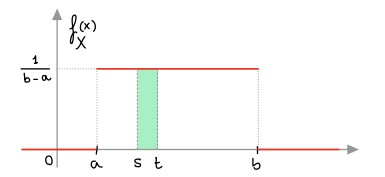
\includegraphics[scale=.8]{Foto/babu.jpg}
\end{figure}

\noindent Dato un intervallo $[s,t] \subseteq [a,b]$  avremo che $$P(X \in [s,t]) = \int_s^t f(x) dx + \dfrac{1}{b-a} = \int_s^t 1 \text{ } dx = \dfrac{t-s}{b-a}$$

\noindent \textbf{Osservazione}: Poiché la variabile aleatoria uniforme continua assume un'infinita quantità di valori in un intervallo continuo [0,3], la probabilità di ottenere un valore specifico x è zero. In altre parole, la probabilità di ottenere un risultato esatto in una variabile aleatoria continua è sempre zero. 

\subsection{Esponenziale}

Una variabile aleatoria \textbf{esponenziale} è spesso utilizzata per descrivere il tempo tra gli arrivi di eventi casuali indipendenti di un processo di Poisson. Misuriamo il tempo medio di evento come $\tau$, avremo che $\lambda = \dfrac{1}{\tau}$. La funzione che la descrive è

\begin{equation}
  f_X(x) =
    \begin{cases}
      \lambda \cdot e^{-\lambda \cdot x}& \text{se } x \geq 0\\
      0 & \text{se } x < 0\\
    \end{cases}       
\end{equation}

\begin{figure}[h!]
    \centering
    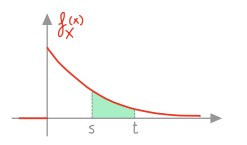
\includegraphics{Foto/bibi.jpg} 
\end{figure}

\noindent Una variabile aleatoria X con tale densità è detta esponenziale di parametro $\lambda \in (0, \infty) $ e si scrive X $\sim$ Exp($\lambda$). Avremo che:
\begin{itemize}
    \item $P(X \in [s,t]) = \int_s^t f_X(x)dx = e^{- \lambda \cdot s} - e^{- \lambda \cdot t}$
    \item $E[X] = \dfrac{1}{\lambda}$
    \item $Var[X] = \dfrac{1}{\lambda^2}$
\end{itemize}
\newpage
\subsection{Normale}

Abbiamo già visto due classi notevoli assolutamente continue: uniforme continua ed esponenziale. Consideriamo ora la più importante: \textbf{variabili aleatorie normali } (o gaussiane).

\noindent Una variabile aleatoria X si dice \textbf{normale standard} e si indica con \newline $Z \sim N(0,1)$ se è assolutamente continua e ha densità: $$f_Z(z) = \dfrac{1}{\sqrt{2 \cdot \pi}} \cdot e^{\left(-\dfrac{z^2}{2} \right)}$$

\begin{figure}[h!]
    \centering
    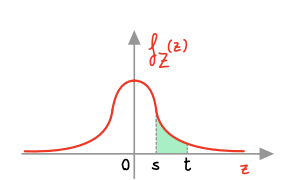
\includegraphics[scale=.8]{Foto/normale.png}
\end{figure}

\noindent Una variabile aleatoria normale standard avrà:
\begin{itemize}
    \item E[Z] = 0
    \item Var[Z] = 1 
    \item P(Z $\in [s,t]) = \displaystyle\int_s^t f_Z(z)dz$
\end{itemize}

\noindent Purtroppo l'integrabile non è calcolabile, allora si introduce la \textbf{funzione di ripartizione di Z} indicata con:  $$ \Phi(z) := F_Z(z) = P(Z \leq z) = \int_s^t f_Z(t)dt$$ Anche questa non è calcolabile esplicitamente ma i valori che può assumere sono riportati in una tabella. \newline

\begin{figure}[h!]
    \centering
    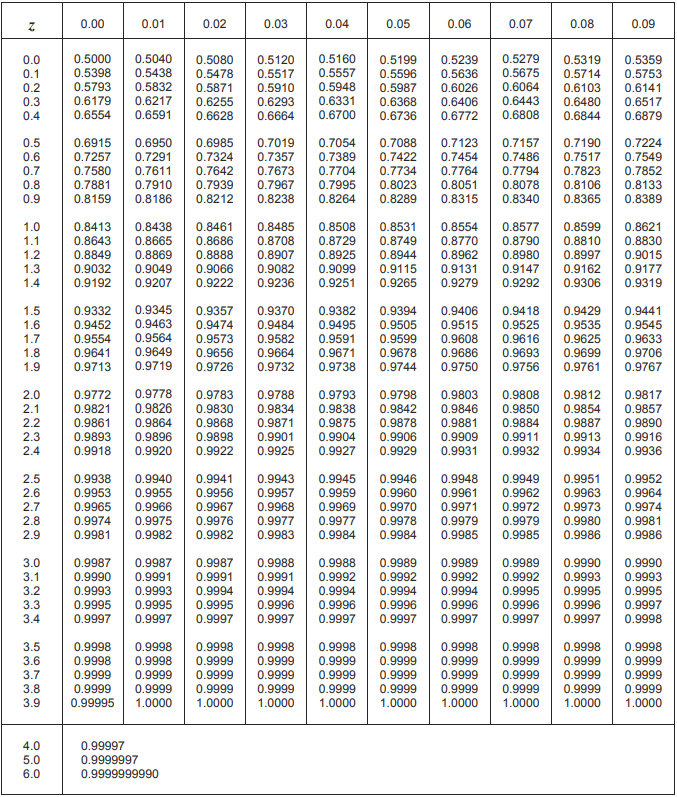
\includegraphics{Foto/tavolameglio.png}
\end{figure} 
\newpage
\noindent \textbf{Osservazione}: per valori negativi si applica la formula: $$\Phi(z) = 1 - \Phi(-z)$$

\newpage
\noindent Una variabile aleatoria X si dice \textbf{normale} con media $\mu$ e varianza $\sigma^2$ e si scrive con $X \sim N(\mu, \sigma^2)$ se X è assolutamente continua con: $$f_X(x) = \dfrac{1}{\sqrt{2 \cdot \pi \cdot \sigma^2}} \cdot e^{-\dfrac({z^2}{2})}$$

\begin{figure}[h!]
    \centering
    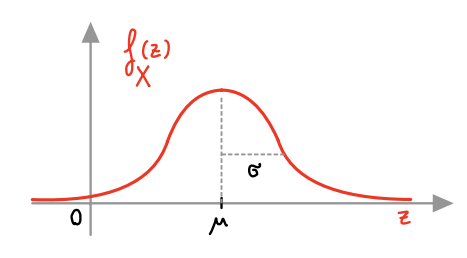
\includegraphics[scale=.7]{Foto/garfichino.png}
    \color{gray}
    \caption{grafico a campana centrato in $\mu$ di ampiezza $\sigma^2$}
\end{figure}

\noindent \textbf{Osservazione}: Ci si può sempre ricondurre da una variabile normale ad una normale standard e viceversa:
\begin{itemize}
    \item $X \sim N(\mu, \sigma^2) \rightarrow{} Z:= \dfrac{X - \mu}{\sigma} \sim N(0,1)$ 
    \item $Z \sim N(0,1) \xrightarrow{} X := \sigma \cdot Z + \mu \sim N(\mu, \sigma^2)$
\end{itemize}

\noindent \textbf{Osservazione}: Da questi trasformazioni, se abbiamo X v.a. normale standard, allora Z v.a. normale ha media $\mu$ e varianza $\sigma^2$: $$X \sim N(\mu, \sigma^2) \rightarrow{} E[Z] = \mu \quad Var[Z] = \sigma^2$$

\subsubsection{Teoremi}
Se X è normale, $Y = a \cdot X + b$ è normale. \newline Se X e Y sono normali indipendenti allora X + Y è normale

\begin{tcolorbox}
    \textbf{Esempio}: $X \sim N(0,1)$, $Y \sim N(0,1)$ allora $$X + Y \sim N(0,2) \qquad X - Y = X + (-1) \cdot (Y) \sim N(0,2)$$
\end{tcolorbox}

\subsubsection{Funzione di ripartizione}

Finora abbiamo studiato le v.a. discrete e assolutamente continue. Introduciamo un nuovo oggetto per v.a. generica: \textbf{funzione di ripartizione} $$F_X(x) := P(X \leq x)$$ 
\begin{itemize}
    \item $F_X$ è ben definita per ogni v.a.
    \item $F_X$ determina la distribuzione della v.a. X: $$P(X \in (s,t]) = F_X(t) - F_X(s)$$
    \item $F_X$ è legata alla densità discreta/densità di X: 
\begin{equation}
  F_X(x) =
    \begin{cases}
        \dsum_{x_i \in ( -\infty, x]} P_X(x_i) & \text{se x è discreta }\\
        \displaystyle\int_{-\infty}^x f_X(t)dt& \text{se x è assolutamente continua }\\
    \end{cases}       
\end{equation}
\end{itemize}

\begin{tcolorbox}
    \textbf{Esempio}: Funzione di ripartizione per variabile discreta: Bernoulli. \newline Sia $X \sim Be(p) \text{ con } p \in (0,1)$: $$X(\Omega) = \{0,1\} \qquad p_X(0) = 1 - p \qquad p_X(1) = p$$ Allora $F_X (x) = P(X \leq x)$ vale:
    \begin{equation}
        f_X(x) =
        \begin{cases}
            0 & \text{se } x < 0\\
            1 - p & \text{se } 0 \leq x < 1 \\
            1 & \text{se } x \geq 1
        \end{cases}       
    \end{equation}
    \end{tcolorbox}
    \begin{figure}[h!]
        \centering
        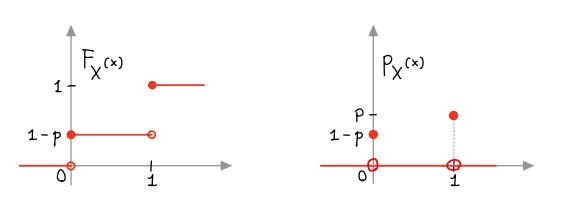
\includegraphics[scale=.6]{Foto/zaza.jpg} 
    \end{figure}


\begin{tcolorbox}
    \textbf{Esempio}: Funzione di ripartizione per variabile uniforme continua \newline Sia $X \sim U(a,b)$: $X(\Omega) = [a,b]$
    \begin{equation}
        f_X(x) = 
        \begin{cases}
            \dfrac{1}{b - a} & \text{ se } a \leq x \leq b \\
            0 & \text{ se } x < a \text{ o } x > b \\
        \end{cases}
    \end{equation}
    Allora $F_X(x) = P(X \leq x)$ vale:
    \begin{equation}
        F_X(x) =
        \begin{cases}
            0 & \text{ se } x < a \\
            \dfrac{x - a}{b - a} & \text{ se } a \leq x \leq b \\
            1  & \text{ se } x > b \\
        \end{cases}
    \end{equation}
\end{tcolorbox}
\begin{figure}[h!]
    \centering
    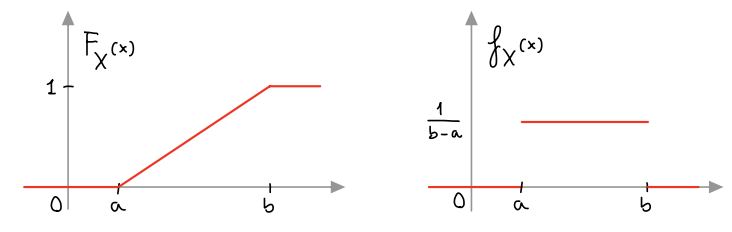
\includegraphics[scale=.7]{Foto/sium.png} 
\end{figure}

\noindent \textbf{Teorema di ripartizione di v.a. discrete} 
\begin{itemize}
    \item X è una variabile aleatoria discreta $\iff$ $F_X$ è costante a tratti 
    \item Valori assunti {$x_i$} $\iff$ punti di discontinuità di $F_X$ 
    \item Densità discreta $\iff$ ampiezze dei salti \item $P_X(x_i) = F_X(x_i) - F_X(x_{\Bar{i}}) $ dove $x_{\Bar{i}} = \lim_{t \xrightarrow{} x_{\Bar{i}}} F_X(t)$
\end{itemize} 

\noindent \textbf{Teorema di ripartizione di v.a. assolutamente continue}
\begin{itemize}
    \item X è una v.a. assolutamente continua (con densità continua a tratti) $\iff$ $F_X$ è una funzione continua ed è derivabile a tratti
    \item Densità $F_X (x) = (F_x)'(x)$
\end{itemize}

\section{Vettori Aleatori}

Abbiamo studiato le v.a. individualmente, ma spesso è interessante lo studio \textit{congiunto} di v.a. relative allo stesso esperimento aleatorio. 
\begin{equation}
  (\Omega, P) =
    \begin{cases}
      X: \Omega \xrightarrow{} \mathbb{R} & \text{variabile aleatoria}\\
      Y: \Omega \xrightarrow{} \mathbb{R} & \text{variabile aleatoria}\\
    \end{cases}       
\end{equation}
La coppia (X,Y) è detta \textbf{vettore aleatorio}: $$(X,Y) : \Omega \xrightarrow{} R^2$$

\subsection{Vettori Aleatori Discreti}

Un vettore $(X,Y)$ si dice \textbf{discreto} se i valori che può assumere sono contenuti in un insieme finito o numerabile $\{(x_i),(y_i)\}$ \newline

\noindent Si definisce \textbf{densità discreta congiunta} come: $$P_{(X,Y)}(x_i, Y_i) := P(X= x_i, Y=y_i) $$

\noindent La relazione tra densità discreta congiunta e la densità discreta delle singole variabili aleatorie è definita come \textbf{densità discreta marginale}: $$P_X(x_i) = \sum_{y_i} P_{(X,Y)}(x_i,y_i) \qquad P_Y(y_i) = \sum_{x_i} P_{(X,Y)}(x_i,y_i)$$

\noindent Il valore medio del prodotto tra due variabili aleatorie discrete X e Y è $$E[X,Y] = \sum_{x_i} \sum_{y_i} x_i \cdot y_i \cdot P_{X,Y}(x_i, y_i)$$

\begin{tcolorbox}
    \textbf{Esempio}: Lancio due monete dove X è prima moneta testa e Z numero totale di teste. \newline $X(\Omega) = {0,1}$ \newline $Y(\Omega) = {0,1,2} \newline p_{(X,Z)}(x,z) = P(X = x, Z = z)$ \newline
    
    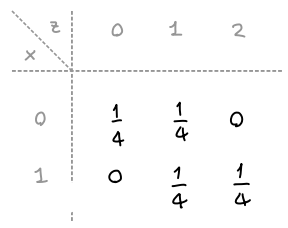
\includegraphics[scale=0.8]{Foto/vettore discreto.png}
\end{tcolorbox}

\subsection{Vettori Aleatori Assolutamente Continui}

Un vettore $(X,Y)$ si dice assolutamente continuo se esiste una funzione $f_{(X,Y)}(x,y) \geq 0$ detta \textbf{densità congiunta} di X e Y tale che $$P(X \in [s,t], Y \in [u,v]) = \int_s^t \left(\int_u^v f_{(X,Y)}(x,y) dy\right) dx$$

\noindent Si definiscono \textbf{densità marginali} come: $$f_X(x) = \int_{-\infty}^{+\infty} f_{(X,Y)}(x,y) dy \quad f_Y(y) = \int_{-\infty}^{+\infty} f_{(X,Y)}(x,y) dx$$

\noindent Il valore medio del prodotto tra due v.a. assolutamente continue X e Y è $$E[X \cdot Y] = \int_{-\infty}^{+\infty} \int_{-\infty}^{+\infty} x \cdot y \cdot f_{(X,Y)}(x,y) \text{ } dx  \text{ } dy$$

\subsection{Indipendenza}

Consideriamo due v.a. X e Y che insieme formano un vettore aleatorio (X,Y). Si dice che X e Y sono \textbf{indipendenti} se $$P(X \in [s,t], Y \in [u,v]) = P(X \in [s,t] \cdot Y \in [u,v])$$

\noindent  Da questa formula si può ricavare che X e Y sono indipendenti se conoscendo il valore che assume Y \textit{non cambia la distribuzione} di X: $$P(X \in [s,t] | Y \in [u,v] ) = P(X \in [s,t]$$

\noindent \textbf{Osservazione}: Per vettori discreti o assolutamente continui, l'indipendenza ha una riformulazione equivalente: $$(X,Y) \text{ discreto, X e Y sono indipendenti sse } p_{X,Y}(x_i,y_i) = p_X(x_i) \cdot p_Y(y_i)$$ $$(X,Y) \text{ assolut. continuo, X e Y sono indipendenti sse } f_{(X,Y)}(x,y) = f(x) \cdot f(y)$$

\noindent \textbf{Osservazione}: Quando le v.a. non sono indipendenti, le densità marginali forniscono meno informazioni della congiunta. Quando le v.a. sono dipendenti, le densità dei singoli fornisce la stessa quantità di informazioni della congiunta. \newline

\noindent Il valore medio del prodotto tra due variabili aleatorie indipendenti X e Y è $$E[X \cdot Y] = E[X] \cdot E[Y]$$

\subsection{Covarianza e Correlazione}

Consideriamo due v.a. X e Y che insieme formano un vettore aleatorio $(X,Y)$. Indichiamo i valori medi con $\mu_X = E[X]$ e $\mu_Y = E[Y]$. \newline Si definisce \textbf{covarianza} di X e Y: $$Cov[X,Y] := E[(X - \mu_X) \cdot (Y - \mu_Y)]$$

\noindent La covarianza misura il \textit{grado di associazione} tra X e Y: \newline $Cov[X,Y] > 0$: a valori grandi di X corrispondono valori grandi di Y \newline  $Cov[X,Y] < 0$: a valori grandi di X corrispondono valori piccoli di Y \newline

\noindent \textbf{Osservazione}: la covarianza si può riscrivere come $$Cov[X,Y] = E[X \cdot Y] - E[X] \cdot E[Y]$$

\subsubsection{Proprietà della covarianza}

\begin{itemize}
    \item Annullamento: $Var[X] = Cov[X, X]$
    \item Simmetria: $Cov[X,Y]= Cov[Y,X]$
    \item Costanti: $Cov[X, c] = 0$
    \item Bilinearità: $Cov[a \cdot X, Y] = a\cdot Cov[X, Y]$ 
    \item Bilinearità: $Cov[X + Z, Y] = Cov[X, Y] + Cov[Z, Y]$
    \item \textbf{Formula della somma}: $Var[X] + Var[Y] + 2 \cdot Cov[X,Y]$
\end{itemize}

\noindent Si definisce \textbf{coefficiente di correlazione lineare}: $$\rho[X,Y] := \dfrac{Cov[X,Y]}{Sd[X] \cdot Sd[Y]}$$ Si tratta di una versione normalizzata della covarianza: 
\begin{itemize}
    \item $-1 \leq \rho[X,Y] \leq 1$
    \item $\rho = \pm 1 \longleftrightarrow Y = a \cdot X + b$
\end{itemize}

\noindent Se Cov[X,Y] = 0, X e Y si dicono \textbf{scorrelate}. \newline

\noindent \textbf{Osservazione}:  Se abbiamo due variabili aleatorie indipendenti, allora sicuramente sono scorrelate, ma \textit{non vale viceversa}

\begin{tcolorbox}
    \textbf{Esempio}: Lancio due dadi regolari a 6 facce. Siano X la somma dei risultati e Y la differenza. Allora X e Y sono scorrelate:
    \begin{equation}
      \begin{aligned}
        Cov[X, Y] & = Cov[A+B, A-B]\\
          & = Cov[A,A] - Cov[A,B] - Cov[B,A] - Cov[B,B]\\
          & = Cov[A,A] - Cov[B,B] \\
          & = Var[A] - Var[B] = 0 
      \end{aligned}
    \end{equation}
    Tuttavia X e Y non sono indipendenti. Per esempio: $$P(X = 12) = \dfrac{1}{6} \quad P(Y = 5) = \dfrac{1}{6}$$ $$P(X = 12, Y = 5) = 0$$ $$ 0 \not= \dfrac{1}{6} \cdot \dfrac{1}{6}$$
\end{tcolorbox}

%-------------Introduzione alla Statistica -----------------------%
\begin{comment}
\section{Verso la Statistica}

Il modello fondamentale per la statistica è una \textbf{sucessione di variabili aleatorie indipendenti e identicamente distribuite (I.I.D.)} \newline

\noindent In un esperimento concreto si osserva una successione di dati numerici $x_1 \cdots x_N$ che interpretiamo come realizzazioni di variabile aleatorie $X_1 \cdots X_N$. \newline 

\noindent Ci poniamo il problema: a partire dai dati $x_1 \cdots x_N$ cosa possiamo dedurre sulla \textit{distribuzione comune} delle v.a. $X_i$?
\end{comment}
%----------------------------------------------------------------%






